\documentclass{article}%
\usepackage[T1]{fontenc}%
\usepackage[utf8]{inputenc}%
\usepackage{lmodern}%
\usepackage{textcomp}%
\usepackage{lastpage}%
\usepackage{authblk}%
\usepackage{graphicx}%
%
\title{X{-}Box Binding Protein 1 (XBP1s) Is a Critical Determinant of Pseudomonas aeruginosa Homoserine Lactone{-}Mediated Apoptosis}%
\author{Thomas Dunn}%
\affil{Program in Developmental Biology, Baylor College of Medicine, Houston, Texas, United States of America}%
\date{01{-}01{-}2005}%
%
\begin{document}%
\normalsize%
\maketitle%
\section{Abstract}%
\label{sec:Abstract}%
There may not be one specific culprit for any systemic intestinal blockage, but that doesn't mean a separate pathway is not useful.\newline%
The substantial blockage  known as extraversion  is caused by areas of the intestinal lining, which literally bent to the predominate shape in the ancestors of millions of years before the species was just a mammal in a cave or tree or bird habitat.\newline%
Studying the intestinal lining tells scientists the body's physiology, and it is used to control cell health and neurobehavior. This genetic activity, called a telomerase, is the blueprint of the intricate networks of fibre{-}coated tissues that provide support to different pathways in the body.\newline%
When patients derive a "terminal" tolerance for certain compounds produced by the telomerase activity in normal and psoriatic human fibroblasts, other cells in the intestinal wall are activated to support normal growth and development.\newline%
The ability to grow and die in a normal environment does not translate into a direct need for medication to block telomerase. If anything, constant vigilance is advisable for patients as telomerase hormone synthesis with the complete distribution of telomerase is inhibited.\newline%
The difference between basing a treatment on the intrinsic biology of a human tumour as determined by the unique telomerase activity in a specific region of the body and the ability to control the synthesis of telomerase is known as differential regulation.\newline%
Improved glycemic control through chemotherapy or immunotherapy, on the other hand, may cut down on the breakdown of telomerase, thus reducing the susceptibility to some common gastrointestinal blockages.\newline%
In addition, for people who have had previous dyscalculia, telomerase function appears to be surprisingly resistant to multiple medications, despite the fact that they have undergone prior surgery.\newline%
Ben Watson, assistant professor of medicine and biomedical sciences, leads the study.\newline%
1. The development of new drugs and medications has increased.\newline%
2. Cell therapies to treat cancers and other disorders are trickier to produce.\newline%
3. The biochemical pathways to cell production and growth are undergoing huge shifts.\newline%
4. Cellular services called dendritic cells are being replaced by invasive "host{-}supporting" growth factors and environmental damage.\newline%
5. Treatment with natural carriers is increasing.\newline%
6. "Trans{-}kidney"{-}organ dysfunction with cellular effects in white blood cells are merging with cancer and other biological processes.\newline%
7. Conventional therapies may be the best way to reduce inflammation and related disease.\newline%
8. Patient behaviors have changed with the use of these medications.\newline%
9. Power plants are disappearing.\newline%
10. Radiation therapy is\newline%
being trialled in children and is gaining acceptance in adults.\newline%
11. The environmental factors that caused the internal damage are not seen in malignant tumors.\newline%
12. Erlichine diacetyl decreases the amount of telomerase produced by normal cells but is not immediately detectable.\newline%
13. Reduced testosterone changes our perception of a "normal" energy level.\newline%
14. Downward temperature is a central control mechanism in our bodies. We don't actually notice changes in the upper respiratory tract.

%
\subsection{Image Analysis}%
\label{subsec:ImageAnalysis}%


\begin{figure}[h!]%
\centering%
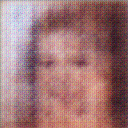
\includegraphics[width=150px]{500_fake_images/samples_5_421.png}%
\caption{A Black And White Photo Of A Black And White Cat}%
\end{figure}

%
\end{document}